\section{Extended Data} \label{sec:extended-data}
\FloatBarrier

\FloatBarrier
% Extended Data Figure 3: Relative success curves
\begin{figure}[h!]
    \centering
    \includegraphics[width=\linewidth]{Figures/indirect-support/real/v1_all-areas.pigean_rs_curves.png}
    \caption{Relative success of PIGEAN-supported target-indication pairs across all clinical areas for common (from curated GWAS and GWAS catalog traits) and rare diseases curated from Orphanet.}
    \label{fig:extended-1}
\end{figure}

% Extended Data Figure 4: Relative success heatmap
\begin{figure}[h!]
    \centering
    \includegraphics[width=\linewidth]{Figures/indirect-support/real/v1_all-areas_relative_success_heatmap.png}
    \caption{Heatmap of the relative success of PIGEAN-supported target-indications as a function of both direct and indirect support across all clinical areas.}
    \label{fig:rs-heatmap}
\end{figure}

\FloatBarrier
% Extended Data Figure 5: Relative success vs indirect support only
\begin{figure}[h!]
    \centering
    \includegraphics[width=\linewidth]{Figures/indirect-support/real/v1_all-areas_relative_success_vs_indirect.png}
    \caption{Relative success as a function of indirect support alone (direct support $\leq$ 5).}
    \label{fig:rs-indirect}
\end{figure}

% Extended Data Figure 6: RS vs mechanistic alignment for best genesets
\begin{figure}[h!]
    \centering
    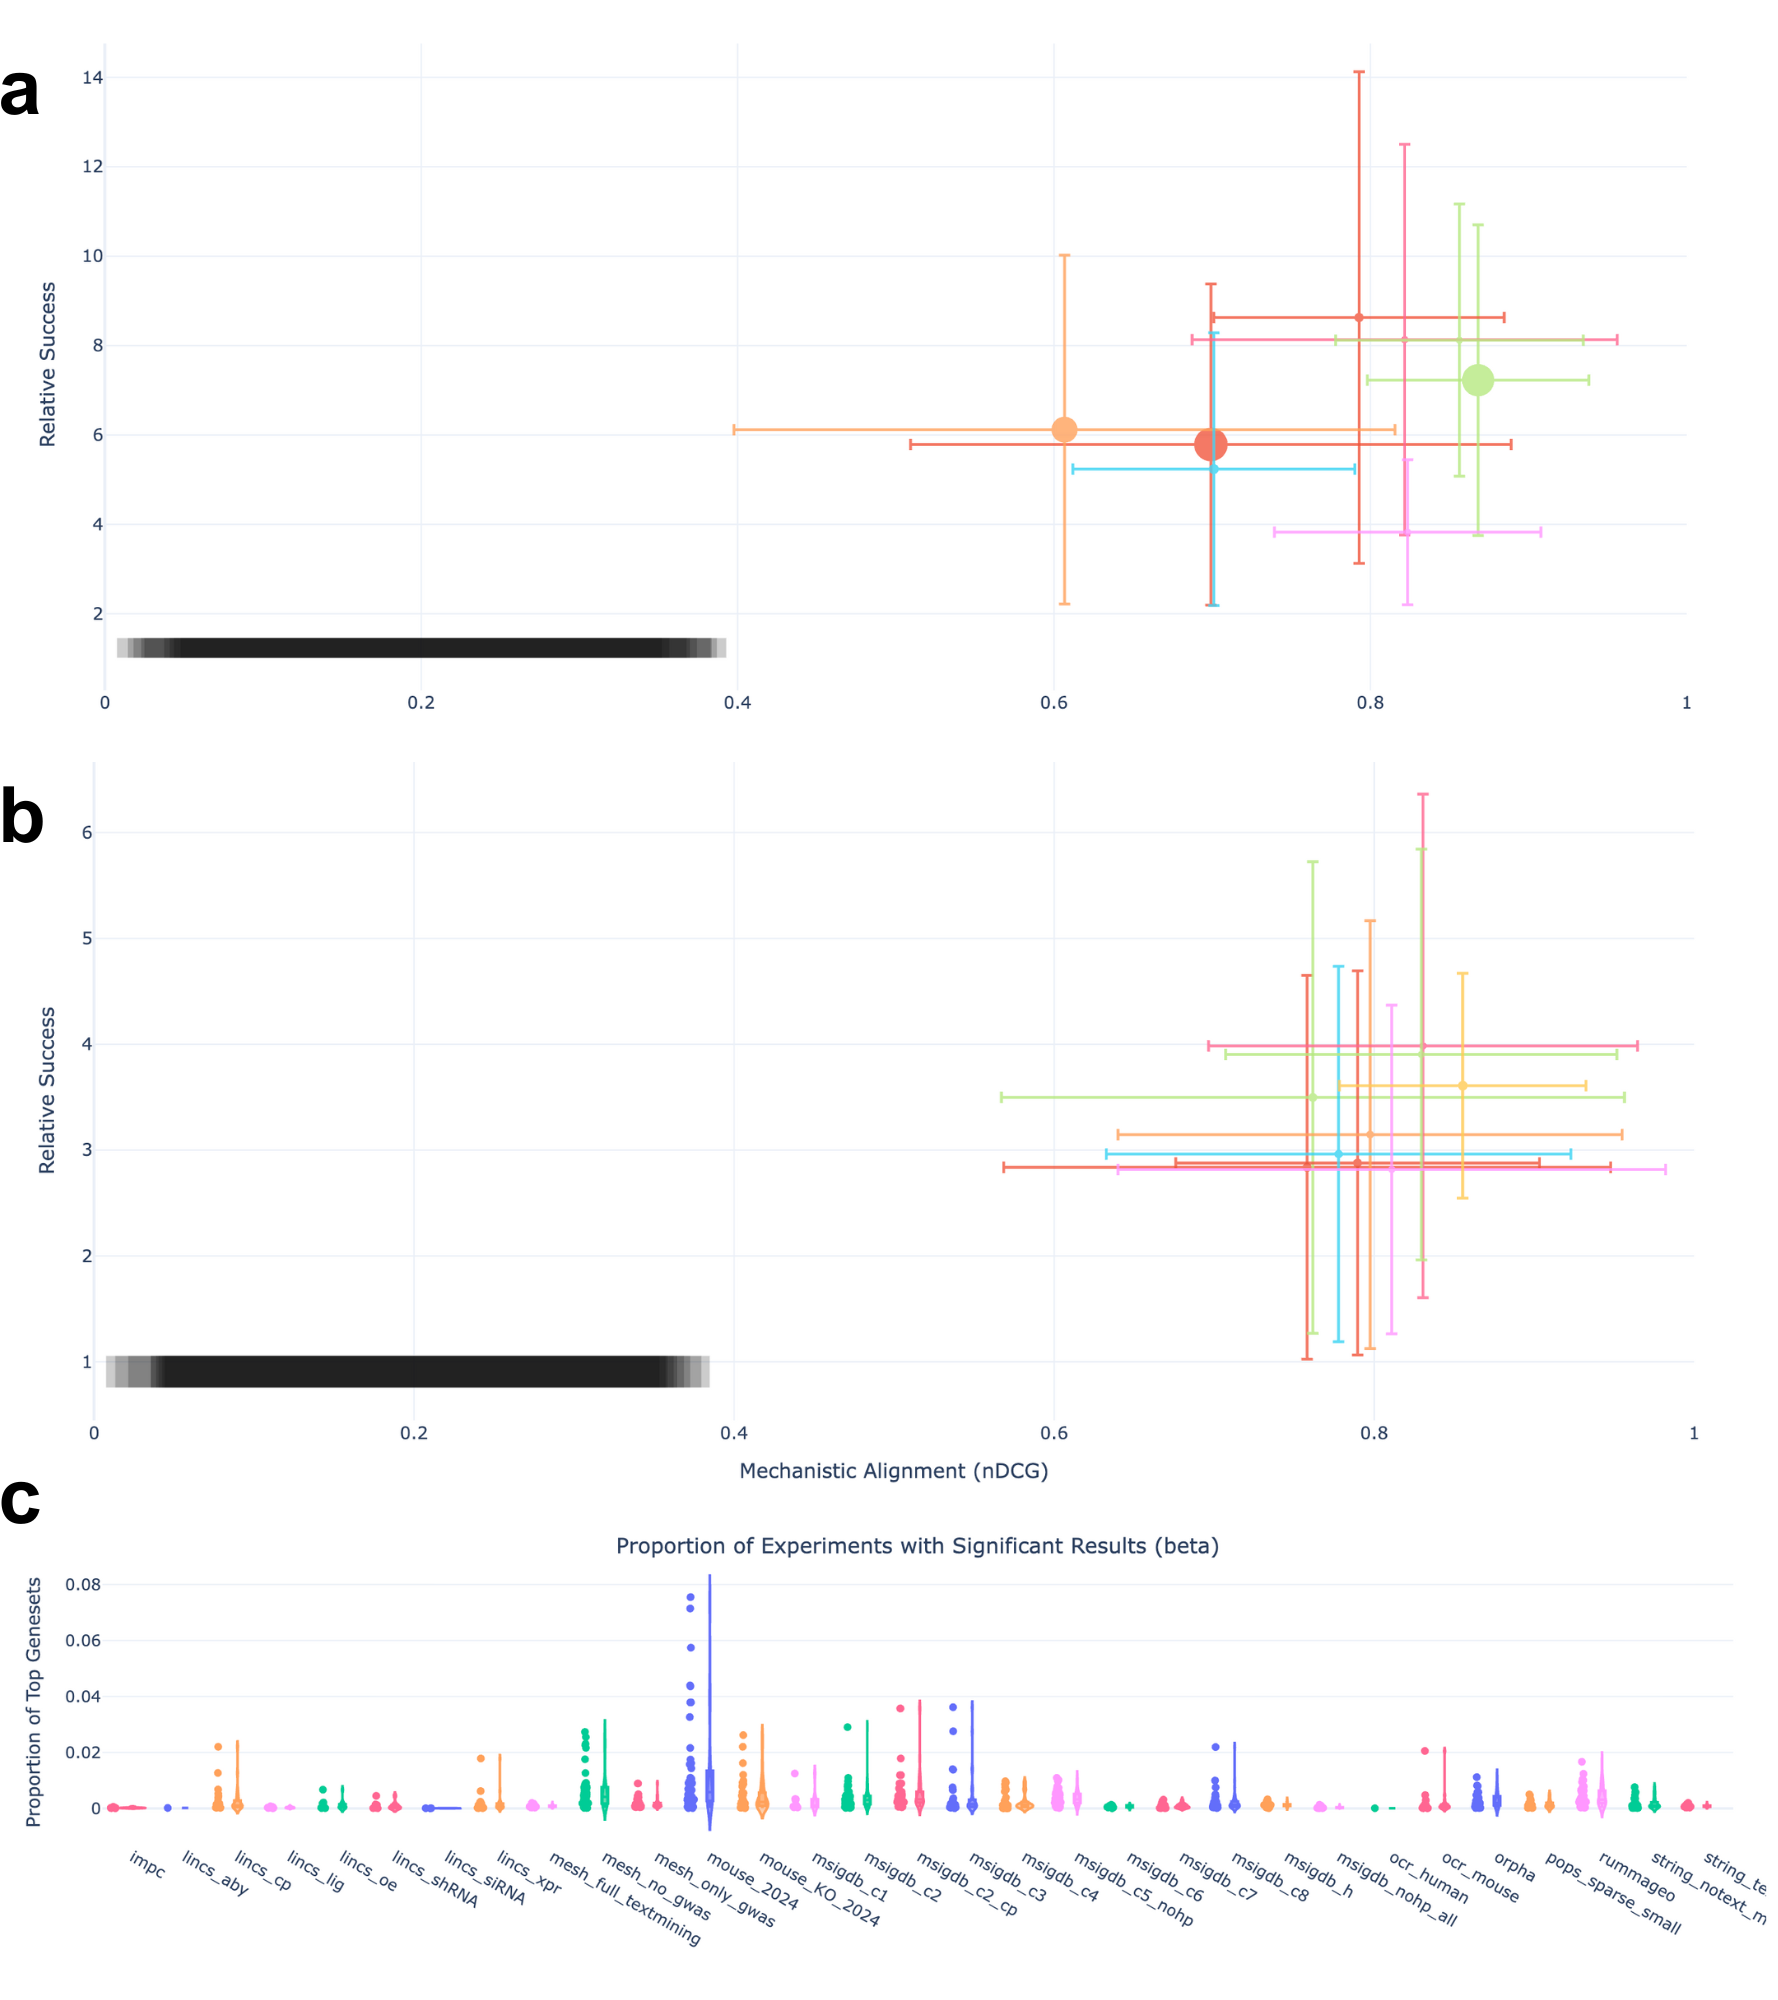
\includegraphics[width=\linewidth]{Figures/indirect-support/real/pigean_rs_vs_ma_best_genesets.png}
    \caption{Relative success versus mechanistic alignment for the best geneset library combinations across validation traits.}
    \label{fig:rs-vs-ma-best-genesets}
\end{figure}

\FloatBarrier
% Extended Data Figure 7: Combined support regression analysis
\begin{figure}[h!]
    \centering
    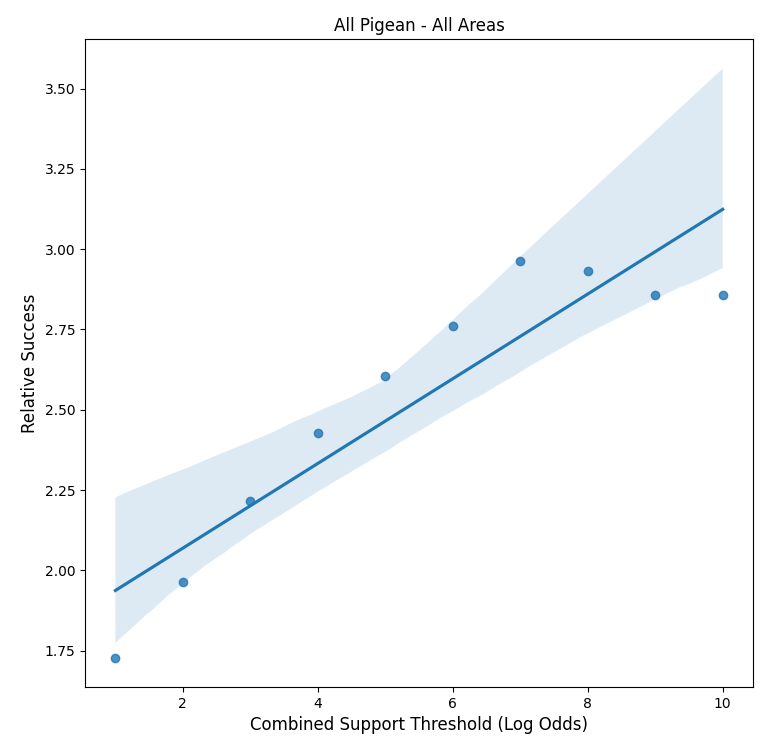
\includegraphics[width=\linewidth]{Figures/indirect-support/real/pigean_combined.regression_analysis.png}
    \caption{Regression analysis of combined PIGEAN genetic support.}
    \label{fig:combined-regression}
\end{figure}

% Extended Data Figure 8: Combined support threshold plot
\begin{figure}[h!]
    \centering
    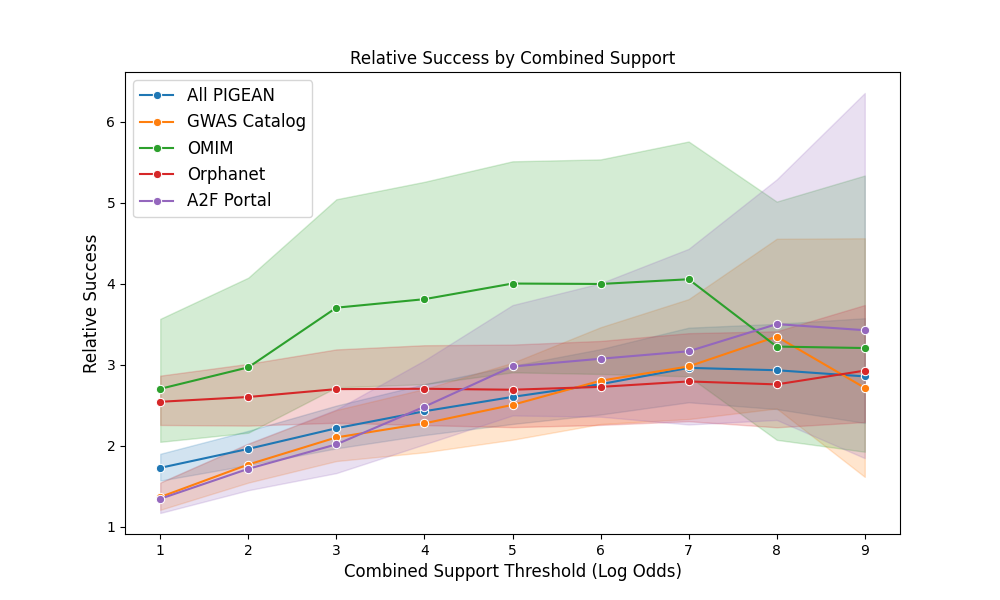
\includegraphics[width=\linewidth]{Figures/indirect-support/real/pigean_combined.threshold_plot.png}
    \caption{Threshold analysis of combined PIGEAN genetic support across varying thresholds.}
    \label{fig:combined-threshold}
\end{figure}

\FloatBarrier
% Extended Data Figure 9: Reproducibility by source
\begin{figure}[h!]
    \centering
    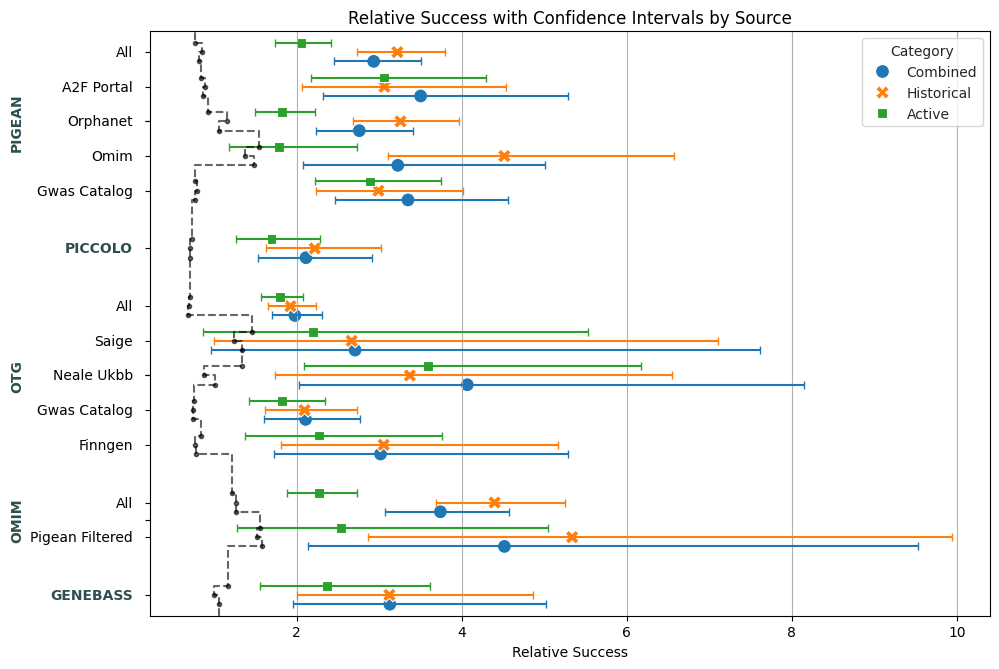
\includegraphics[width=\linewidth]{Figures/indirect-support/real/reproducibility.performance_by_source.png}
    \caption{Reproducibility of PIGEAN performance stratified by annotation source.}
    \label{fig:reproducibility-by-source}
\end{figure}

% Extended Data Figure 10: Rare disease validation
\begin{figure}[h!]
    \centering
    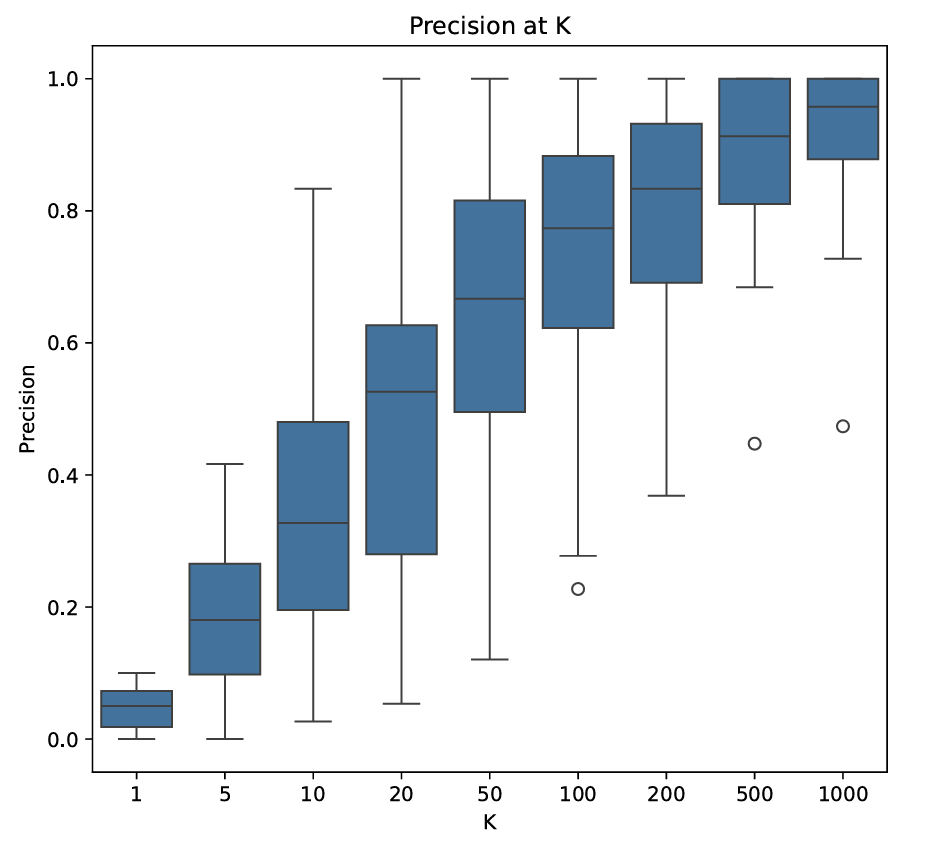
\includegraphics[width=\linewidth]{Figures/indirect-support/real/rare-disease-validation.png}
    \caption{Rare disease validation results for PIGEAN indirect support.}
    \label{fig:rare-disease-validation}
\end{figure}

\FloatBarrier
% Extended Data Figure: Pleiotropy violin plots by LOEUF category
\begin{figure}[h!]
    \centering
    \begin{subfigure}{\textwidth}
        \centering
        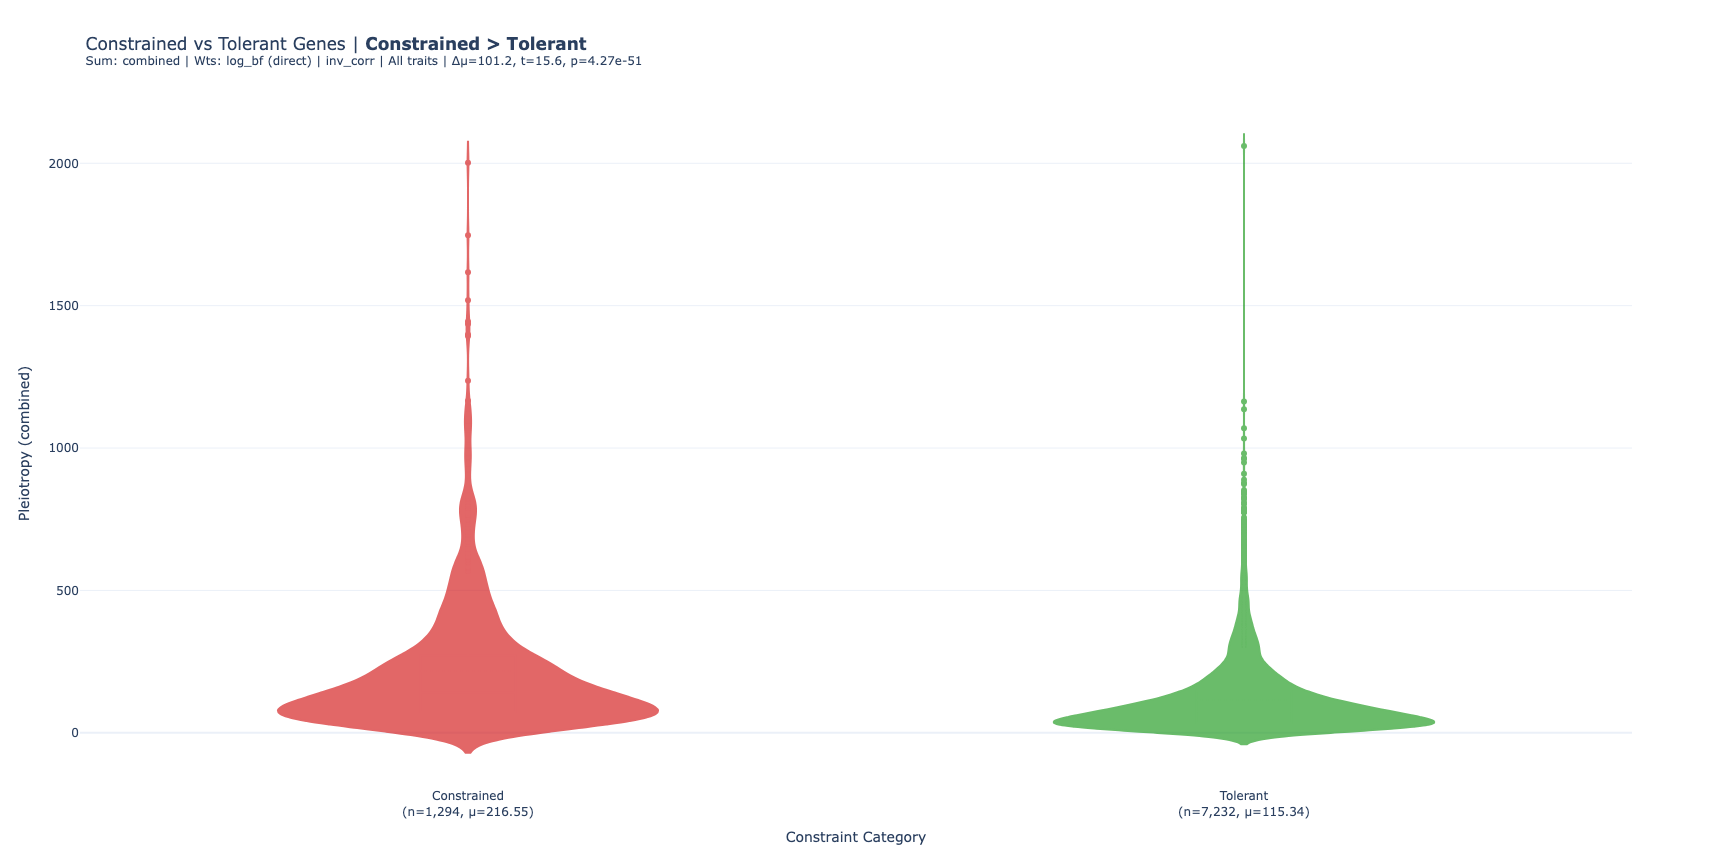
\includegraphics[width=\linewidth]{Figures/indirect-support/real/pleiotropy-violin-all-traits.png}
        \caption{All traits}
        \label{fig:pleiotropy-violin-all}
    \end{subfigure}
    \vspace{0.5em}
    \begin{subfigure}{\textwidth}
        \centering
        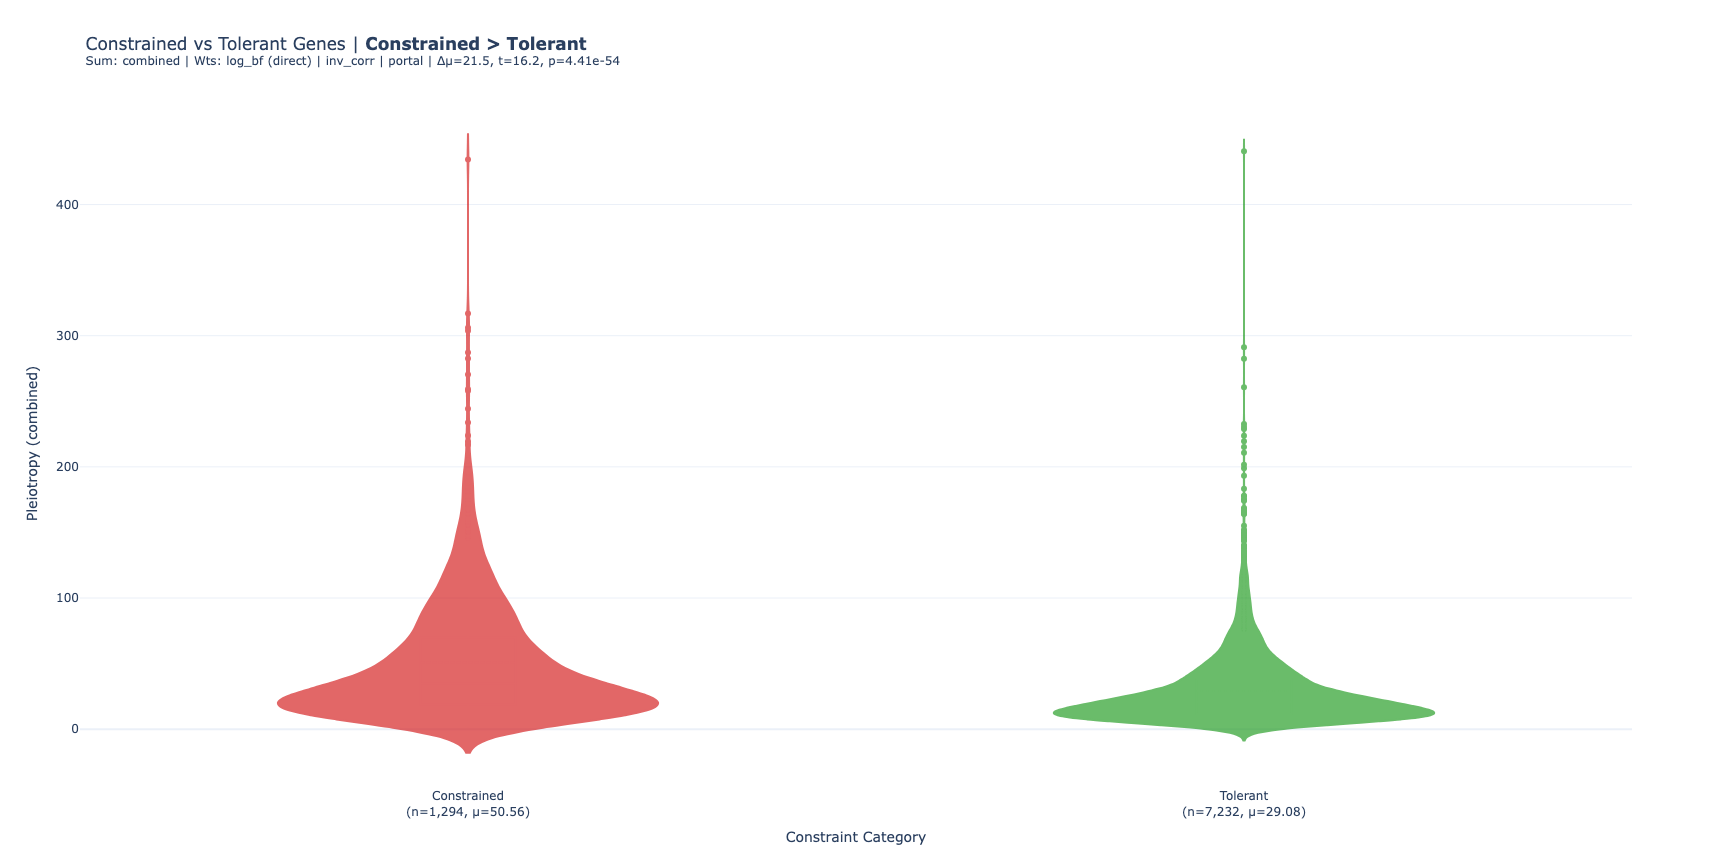
\includegraphics[width=\linewidth]{Figures/indirect-support/real/pleiotropy-violin-portal.png}
        \caption{Portal traits}
        \label{fig:pleiotropy-violin-portal}
    \end{subfigure}
    \vspace{0.5em}
    \begin{subfigure}{\textwidth}
        \centering
        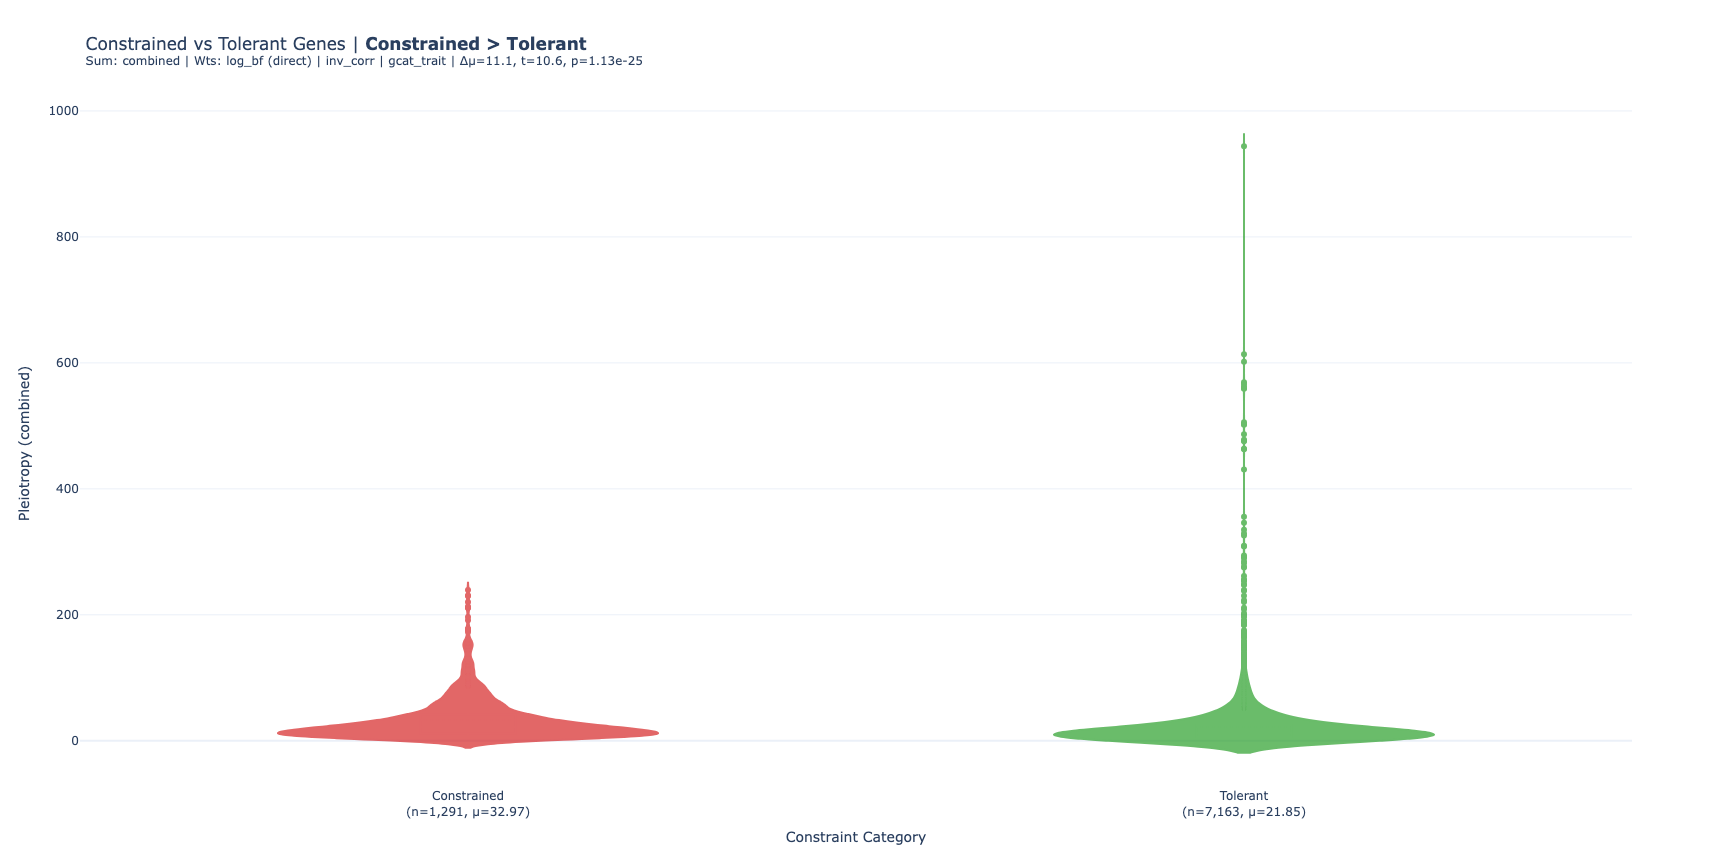
\includegraphics[width=\linewidth]{Figures/indirect-support/real/pleiotropy-violin-gcat.png}
        \caption{GWAS catalog traits}
        \label{fig:pleiotropy-violin-gcat}
    \end{subfigure}
    \vspace{0.5em}
    \begin{subfigure}{\textwidth}
        \centering
        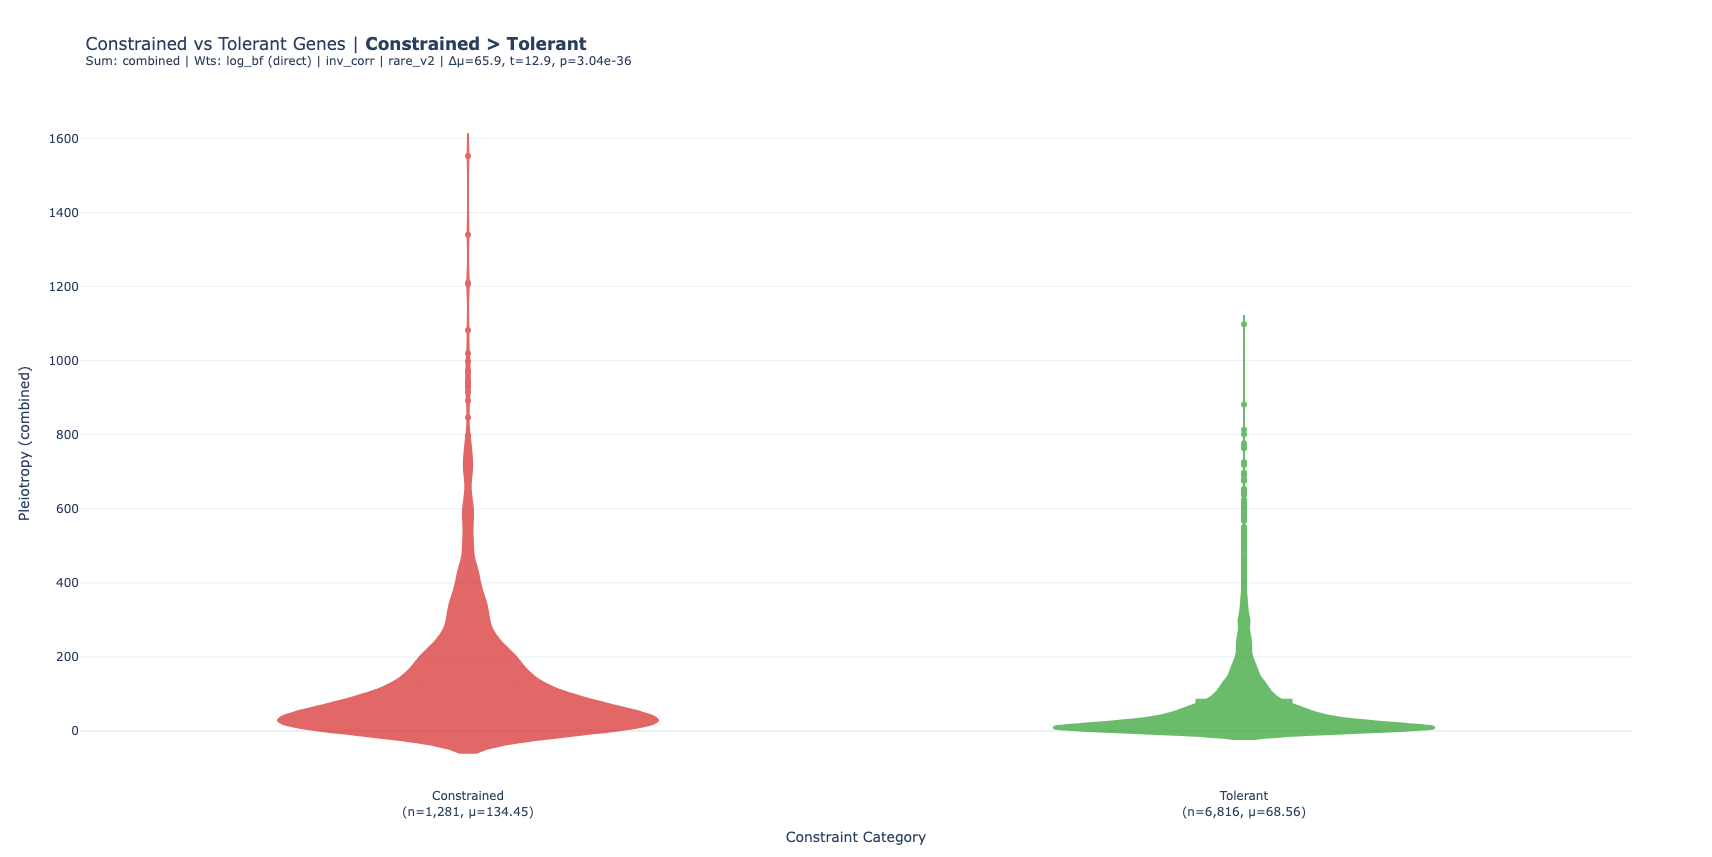
\includegraphics[width=\linewidth]{Figures/indirect-support/real/pleiotropy-violin-rare.png}
        \caption{Rare disease traits}
        \label{fig:pleiotropy-violin-rare}
    \end{subfigure}
    \caption{Distribution of PIGEAN-derived pleiotropy scores for constrained (LOEUF $< 0.35$) versus tolerant (LOEUF $> 1.0$) genes across trait categories. Constrained genes show significantly higher pleiotropy across all score types (combined, direct, indirect) and all trait groups (all $P < 10^{-12}$).}
    \label{fig:pleiotropy-violin}
\end{figure}

\FloatBarrier
% Extended Data Table: Pleiotropy-Constraint Correlation
\begin{table}[h!]
\centering
\caption{Correlation between gene pleiotropy and evolutionary constraint across PIGEAN evidence types and trait groups. Pleiotropy was computed as the inverse-correlation-weighted sum of positive Bayes factors across 3{,}026 traits (18{,}325 genes), with trait correlation weights derived from direct Bayes factors. Effective trait counts: combined $N_\text{eff}$ = 130, direct $N_\text{eff}$ = 311, indirect $N_\text{eff}$ = 61. $\rho$: Spearman rank correlation; $R^2$: Pearson coefficient of determination. All $P < 10^{-5}$ except entries marked $\dagger$ ($P > 0.05$). $N \approx 15{,}800$ genes per test.}
\label{tab:pleiotropy_constraint}
\small
\begin{tabular}{llrrrrrrrr}
\hline
& & \multicolumn{2}{c}{\textbf{LOEUF}} & \multicolumn{2}{c}{\textbf{lof\_z}} & \multicolumn{2}{c}{\textbf{mis\_z}} & \multicolumn{2}{c}{\textbf{syn\_z}} \\
\cmidrule(lr){3-4} \cmidrule(lr){5-6} \cmidrule(lr){7-8} \cmidrule(lr){9-10}
\textbf{Evidence} & \textbf{Traits} & $\rho$ & $R^2$ & $\rho$ & $R^2$ & $\rho$ & $R^2$ & $\rho$ & $R^2$ \\
\hline
Combined & All          & $-$0.261 & 0.050 & 0.250 & 0.050 & 0.171 & 0.025 & 0.009$^\dagger$    & $<$0.001 \\
         & Portal       & $-$0.247 & 0.054 & 0.243 & 0.058 & 0.125 & 0.010 & $-$0.024           & 0.003 \\
         & GWAS catalog & $-$0.208 & 0.012 & 0.194 & 0.010 & 0.122 & 0.004 & $-$0.039           & $<$0.001 \\
         & Rare         & $-$0.206 & 0.034 & 0.197 & 0.034 & 0.164 & 0.023 & 0.045              & $<$0.001 \\
\hline
Direct   & All          & $-$0.252 & 0.047 & 0.250 & 0.052 & 0.136 & 0.014 & $-$0.018$^\dagger$ & $<$0.001 \\
         & Portal       & $-$0.222 & 0.042 & 0.219 & 0.046 & 0.101 & 0.004 & $-$0.028           & 0.004 \\
         & GWAS catalog & $-$0.155 & 0.010 & 0.145 & 0.010 & 0.054 & $<$0.001 & $-$0.081        & 0.002 \\
         & Rare         & $-$0.163 & 0.020 & 0.171 & 0.024 & 0.126 & 0.014 & 0.038              & $<$0.001 \\
\hline
Indirect & All          & $-$0.214 & 0.037 & 0.200 & 0.034 & 0.159 & 0.024 & 0.023$^\dagger$    & $<$0.001 \\
         & Portal       & $-$0.243 & 0.033 & 0.230 & 0.035 & 0.159 & 0.016 & $-$0.013$^\dagger$ & $<$0.001 \\
         & GWAS catalog & $-$0.233 & 0.007 & 0.214 & 0.006 & 0.169 & 0.006 & 0.003$^\dagger$    & $<$0.001 \\
         & Rare         & $-$0.189 & 0.032 & 0.178 & 0.029 & 0.152 & 0.022 & 0.041              & $<$0.001 \\
\hline
\end{tabular}
\end{table}

% Extended Data Table: Uncorrected Beta Geneset Pleiotropy (2x2 panel layout)
\FloatBarrier
\begin{table*}[h!]
\caption{Top pleiotropic gene sets across trait-group stratifications in the Mouse+MSigDB model (uncorrected $\beta_\text{uncorrected}$ score). Values are inverse-correlation-weighted pleiotropy sums with posterior-transformed Bayes factors.}
\label{tab:supp-top-geneset-pleiotropy-beta-uncorrected-longtable}
\centering
\small
\setlength{\tabcolsep}{3pt}
\renewcommand{\arraystretch}{1.05}
\begin{tabular}{@{} r @{\;\;} p{0.34\textwidth} r @{\qquad} r @{\;\;} p{0.34\textwidth} r @{}}
\toprule
\multicolumn{3}{@{}l}{\textbf{(a) All traits}} & \multicolumn{3}{l@{}}{\textbf{(b) GWAS catalog traits}} \\
\cmidrule(r){1-3}\cmidrule(l){4-6}
 & \textbf{Gene set} & \textbf{Score} &  & \textbf{Gene set} & \textbf{Score} \\
\midrule
1 & CASP3\_TARGET\_GENES & 310.3 & 1 & REACTOME\_PLASMA\_LIPOPROTEIN\_REMODELING & 236.9 \\
2 & WP\_CILIOPATHIES & 287.2 & 2 & WP\_STATIN\_INHIBITION\_OF\_CHOL\_PRODUCTION & 207.9 \\
3 & WP\_BARDET\_BIEDL\_SYNDROME & 285.9 & 3 & GOBP\_PROTEIN\_CONTAINING\_COMPLEX\_REMOD & 204.7 \\
4 & REACTOME\_PLASMA\_LIPOPROTEIN\_REMODELING & 285.4 & 4 & GOBP\_ACYLGLYCEROL\_HOMEOSTASIS & 199.9 \\
5 & MT & 285.1 & 5 & REACTOME\_PLASMA\_LIPOPROTEIN\_ASSEMBLY\dots & 199.1 \\
6 & WP\_CHOLESTEROL\_METABOLISM & 262.8 & 6 & GOBP\_PROTEIN\_LIPID\_COMPLEX\_ORGANIZATION & 198.0 \\
7 & WP\_STATIN\_INHIBITION\_OF\_CHOL\_PRODUCTION & 262.6 & 7 & GOCC\_HIGH\_DENSITY\_LIPOPROTEIN\_PARTICLE & 188.0 \\
8 & WP\_JOUBERT\_SYNDROME & 254.9 & 8 & WP\_CHOLESTEROL\_METABOLISM & 185.4 \\
9 & WP\_PRIMARY\_CILIUM\_DEV\_CRISPR & 251.6 & 9 & GOBP\_REG\_PLASMA\_LIPOPROTEIN\_LEVELS & 184.1 \\
10 & GOBP\_PROTEIN\_CONTAINING\_COMPLEX\_REMOD & 249.4 & 10 & GOBP\_CHOLESTEROL\_EFFLUX & 173.6 \\
\midrule
\multicolumn{3}{@{}l}{\textbf{(c) Portal traits}} & \multicolumn{3}{l@{}}{\textbf{(d) Rare disease traits}} \\
\cmidrule(r){1-3}\cmidrule(l){4-6}
 & \textbf{Gene set} & \textbf{Score} &  & \textbf{Gene set} & \textbf{Score} \\
\midrule
1 & GOBP\_CARDIAC\_CHAMBER\_MORPHOGENESIS & 45.9 & 1 & CASP3\_TARGET\_GENES & 310.3 \\
2 & mp\_short\_ulna & 45.8 & 2 & WP\_CILIOPATHIES & 287.1 \\
3 & mp\_abnormal\_cartilage\_development & 45.6 & 3 & WP\_BARDET\_BIEDL\_SYNDROME & 285.4 \\
4 & GOBP\_CHONDROCYTE\_DIFFERENTIATION & 44.5 & 4 & MT & 285.1 \\
5 & WP\_STATIN\_INHIBITION\_OF\_CHOL\_PRODUCTION & 43.0 & 5 & WP\_JOUBERT\_SYNDROME & 254.9 \\
6 & mp\_abnormal\_xiphoid\_process\_morphology & 42.9 & 6 & WP\_PRIMARY\_CILIUM\_DEV\_CRISPR & 251.6 \\
7 & mp\_short\_humerus & 42.2 & 7 & GOCC\_CILIARY\_TRANSITION\_ZONE & 244.3 \\
8 & GOBP\_REG\_CHONDROCYTE\_DIFFERENTIATION & 41.0 & 8 & mp\_preaxial\_polydactyly & 229.3 \\
9 & GOBP\_CARDIAC\_SEPTUM\_MORPHOGENESIS & 39.8 & 9 & TFAM\_TARGET\_GENES & 213.5 \\
10 & mp\_abnormal\_cartilage\_morphology & 39.8 & 10 & HJURP\_TARGET\_GENES & 209.0 \\
\bottomrule
\end{tabular}
\end{table*}

% Force all extended data floats to be placed before supplementary figures begin
\clearpage

% --- Supplementary Simulation Figures ---

% Supplementary Figure 1: Null simulation results
\begin{figure}[h!]
    \centering
    
\includegraphics[width=\linewidth]{Figures/indirect-support/real/suppfig1.png}
    \caption{Null simulation results. (a) Inferred gene annotation effect sizes under null GWAS. (b-d) Indirect, direct, and combined gene ABFs under null GWAS. (e) Annotation effect sizes with permuted gene annotations on real GWAS. (f) Maximum annotation effect size with permuted annotations. (g-h) Combined and direct gene ABFs under null simulations.}
    \label{fig:null_sim}
\end{figure}

% Supplementary Figure 2: Non-null simulation accuracy
\begin{figure}[h!]
    \centering
    
\includegraphics[width=\linewidth]{Figures/indirect-support/real/suppfig2.png}
    \caption{Non-null simulation accuracy. (a) Estimated vs. true annotation effect sizes. (b) Estimated vs. true gene ABFs. (c-d) Asymmetric shrinkage of negative vs. positive annotation effects and gene ABFs.}
    \label{fig:non_null_sim}
\end{figure}

% Supplementary Figure 3: Simulation parameter sensitivity
\begin{figure}[h!]
    \centering
    
\includegraphics[width=\linewidth]{Figures/indirect-support/real/suppfig3.png}
    \caption{Effect of simulation parameters on PIGEAN accuracy. (a) Accuracy as a function of effect size magnitude ($\sigma$). (b) Accuracy as a function of sparsity ($p$). (c) Effect of noise on ABF and annotation effect size accuracy.}
    \label{fig:sim_params}
\end{figure}

% Supplementary Figure 4: Gibbs sampling stability
\begin{figure}[h!]
    \centering
    
\includegraphics[width=\linewidth]{Figures/indirect-support/real/suppfig4.png}
    \caption{Stability of PIGEAN estimates across Gibbs sampling runs with varying numbers of iterations and chains.}
    \label{fig:sim_stability}
\end{figure}

% Supplementary Figure 5: Joint vs one-step inference
\begin{figure}[h!]
    \centering
    
\includegraphics[width=\linewidth]{Figures/indirect-support/real/suppfig5.png}
    \caption{Comparison of full joint inference (iterative re-estimation of gene and gene set values) versus one-step estimation of gene set effect sizes.}
    \label{fig:sim_onestep}
\end{figure}

% Supplementary Figure 6: w-parameter regularization
\begin{figure}[h!]
    \centering
    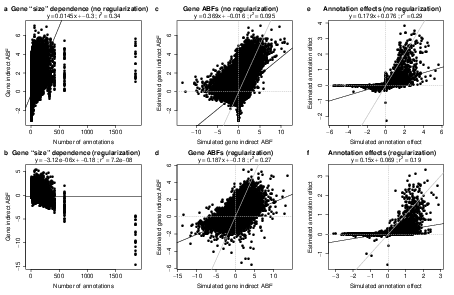
\includegraphics[width=\linewidth]{Figures/indirect-support/real/suppfig6.png}
    \caption{Effect of the $w$ regularization parameter on annotation effect size estimation accuracy.}
    \label{fig:sim_reg}
\end{figure}

% Supplementary Figure 7: Alpha regularization (induced bias)
\begin{figure}[h!]
    \centering
    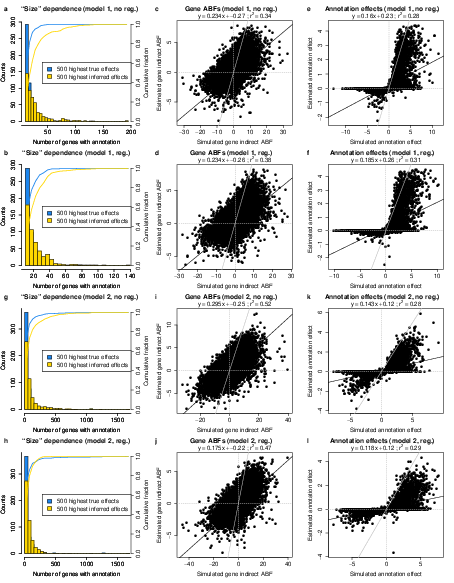
\includegraphics[width=\linewidth]{Figures/indirect-support/real/suppfig7.png}
    \caption{Importance of $\alpha$ regularization to penalize well-annotated genes. Biases and ABF accuracy reductions induced by asymmetric annotation standard errors are corrected by the $\alpha$ parameter.}
    \label{fig:sim_induced}
\end{figure}

% Supplementary Figure 8: Sparsity parameter inference
\begin{figure}[h!]
    \centering
    
\includegraphics[width=\linewidth]{Figures/indirect-support/real/suppfig8.png}
    \caption{Inference of PIGEAN's sparsity parameter ($p$) from simulated data.}
    \label{fig:sim_param_infer}
\end{figure}

% Supplementary Figure 9: Varying sigma sensitivity
\begin{figure}[h!]
    \centering
    
\includegraphics[width=\linewidth]{Figures/indirect-support/real/suppfig9.png}
    \caption{Sensitivity of PIGEAN estimation accuracy to varying the shrinkage parameter $\sigma$ from its simulated value.}
    \label{fig:sim_vary_sigma}
\end{figure}

% Supplementary Figure 10: Varying p sensitivity
\begin{figure}[h!]
    \centering
    
\includegraphics[width=\linewidth]{Figures/indirect-support/real/suppfig10.png}
    \caption{Sensitivity of PIGEAN estimation accuracy to varying the sparsity parameter $p$ from its simulated value.}
    \label{fig:sim_vary_p}
\end{figure}

% Supplementary Figure 11: GWAS association noise impact
\begin{figure}[h!]
    \centering
    
\includegraphics[width=\linewidth]{Figures/indirect-support/real/suppfig11.png}
    \caption{Impact of association noise on PIGEAN performance with GWAS summary statistics. (a) Observed vs. true disease probabilities. (b) Effect of perfect SNP-to-gene linkages. (c) Effect of reduced annotation noise. (d) Effect of larger sample sizes. (e) Marginal vs. joint annotation effect accuracy. (f) Effect of inferring regularization parameters.}
    \label{fig:sim_gwas_gene_set}
\end{figure}

% Supplementary Figure 12: Additional simulation figure
\begin{figure}[h!]
    \centering
    
\includegraphics[width=\linewidth]{Figures/indirect-support/real/suppfig12.png}
    \caption{Additional simulation results.}
    \label{fig:suppfig12}
\end{figure}
